%*****************************************
\chapter{Der Soziale Netzwerke Vergleich}\label{ch:vergleich}
%*****************************************

Im vorherigen Teil der Arbeit haben wir uns damit beschäftigt, wie soziale Netzwerke so gut und realitätsnah wie möglich konstruiert werden können. Wir haben Analysen durchgeführt und festgestellt, dass die Werte unserer \textbf{Grad-} und \textbf{Nähe-Zentralität} näherungsweise normalverteilt sind. Daher liegt es nahe, weitere sozialen Netzwerke und ihre Analysen zum Vergleich heranzuziehen. Leitfragen sind hierbei, was zu erwarten ist, ob die Ergebnisse den Erwartungen entsprechen oder sogar widersprechen und warum dies der Fall ist. Zusätzlich möchten wir optimalerweise eine Möglichkeit erarbeitet, wie wir unsere Graphen bzw. die Generierung angepasst könnten um möglicherweise noch bessere Graphen zu erhalten, die die sozialen Netzwerken noch mehr ähneln. 

\section{Der Datensatz und die Analyse}
Auf der Suche nach vergleichbaren sozialen Netzwerken, beziehungsweise Datensätzen, ist die Suche scheinbar endlos. Auf vielen Webseiten sind große Datensätze für alle Nutzer*innen zugänglich. Meistens als \textbf{CSV} Datei, welche ideal zur Erstellung von Graphen mit unserem Generator geeignet sind. In diesem Teil der Arbeit betrachten wir mehrere Datensätze. Natürlich aufgrund der Tatsache, dass sie spannend sind aber auch um mehrere Vergleichswerte zu haben. Starten wir zunächst mit den Daten \cite{GOT} von unserem \textbf{Game of Thrones} Plot \ref{fig:GameOfThrones}. Da wir bereit die Analyse der \textbf{Zentralitäten} und die generelle visuelle Analyse des Graphen durchgeführt haben, reicht uns nun lediglich die Verteilung der Zentralitäten zu betrachten. Die Tabelle mit den Werten der Zentralitätsberechnungen befinden sich erneut in \cite{TZ}. Nachdem wir den Datensatz als \textbf{CSV} Datei in unserem Generator eingelesen und anschließend geplottet haben, konnten wir den folgenden Graphen konstruiert:

\FloatBarrier
\begin{figure}[h!]%
  \centering
  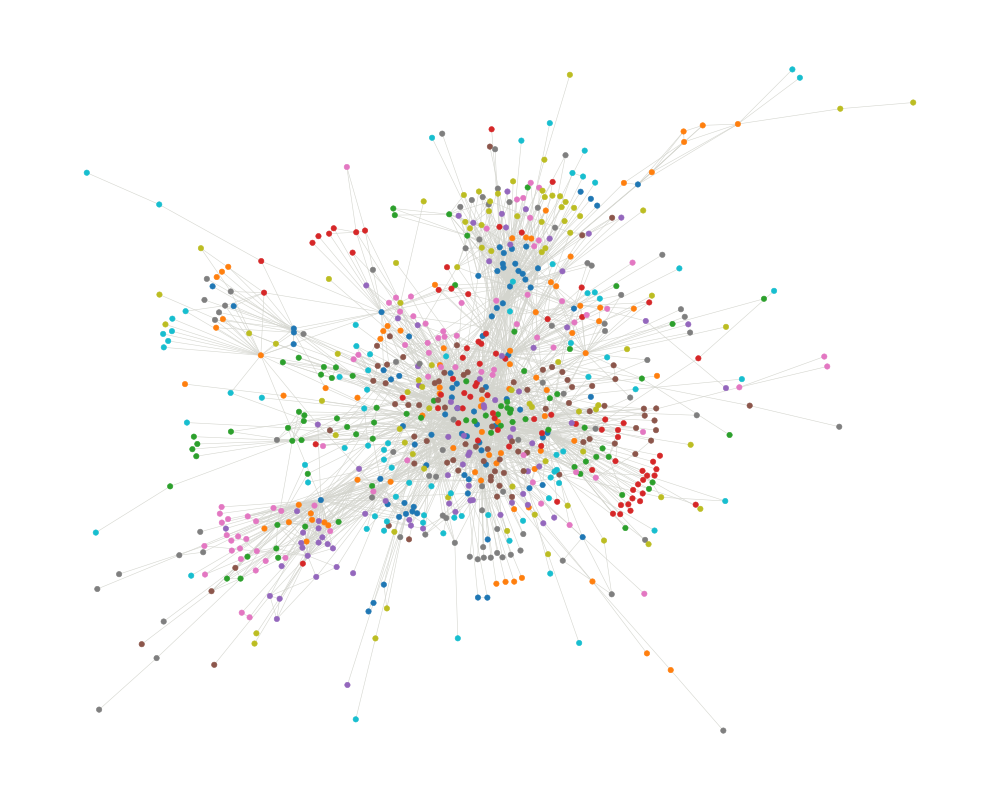
\includegraphics[width=0.7\textwidth]{Graphics/GOTPlot.png}
  \caption{Game of Thrones Graph 2.0, \\
  selbst erstellt}
  \label{fig:GOT2.0}
\end{figure}
\FloatBarrier

Diesen Plot lassen beabsichtigt unkommentiert, da wir ihn lediglich zur Argumentation für die Verteilung der Zentralitäten benötigen und daher die visuelle Form des Graphen nur von zweitrangiger Bedeutung für uns ist. Zudem ist zu vermerken, dass der eigentliche Datensatz gewichtet ist, und unser Graph daher bereits schon visuell nicht dem Graphen aus \ref{fig:GameOfThrones} ähnelt. Jedoch ist es sinnvoll die Gewichte außen vor zu lassen, da wir in dieser Arbeit ausschließlich ungewichtete Graphen nachbilden. Nachdem wir die Daten des Graphen \ref{fig:GOT2.0} eingelesen, die Zentralitäten berechnet haben und anschließend den Balkengraphen erstellt haben, ist folgender Plot entstanden:

\FloatBarrier
\begin{figure}[h!]%
  \centering
   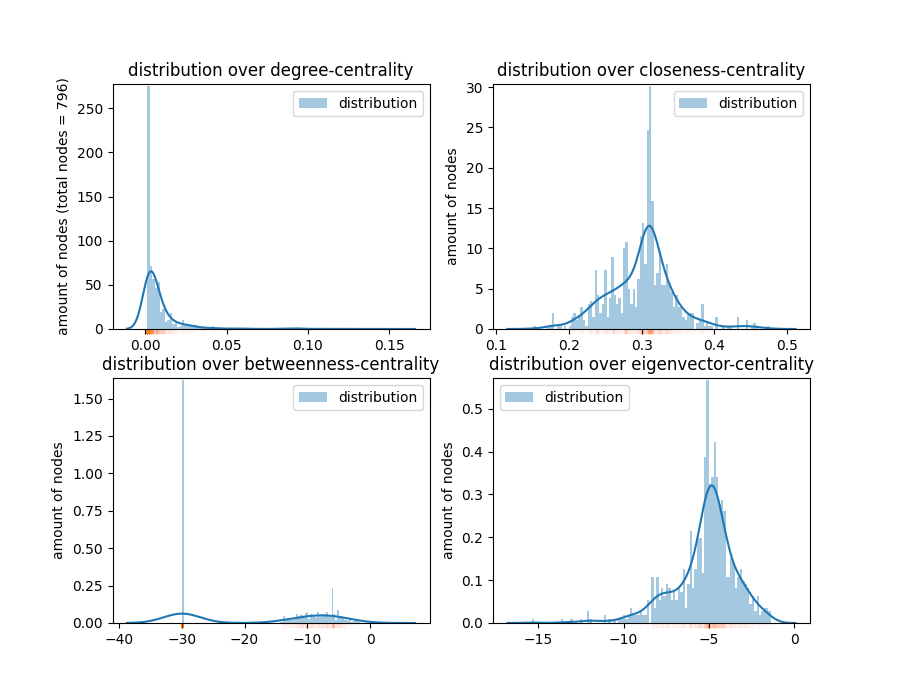
\includegraphics[width=0.8\textwidth]{Graphics/GOT-Distribution.png}
  \caption{Game of Thrones Verteilung der Zentralitäten}
  \label{fig:distributionGOT}
\end{figure}
\FloatBarrier
 
 Auf den ersten Blick können wir bereits feststellen, dass wir andere Ergebnisse erwartet haben. Einzig die Verteilung der \textbf{Nähe-Zentralität} ähnelt der erwarteten Normalverteilung. Die \textbf{Betweenness-} und \textbf{Eigenvektor-Zentralität} hingegen ähneln zwar nicht exakt dem, was wir in \ref{fig:distributionALL} herausgefunden haben aber ziehen auf jeden Fall Parallelen. Denn beide haben einen Ausschlag von mindestens einem Balken, was wir schon im vorherigen Kapitel damit begründet haben, dass es die Folge davon ist, wenn viele kürzeste Wege stets über die gleichen
Knoten verlaufen, wir also keine Alternativen im Graph haben. Die \textbf{Grad-Zentralität} hingegen darf uns verwundern. Sie ähnelt keinesfalls der Normalverteilung aber sieht sehr nach einer Exponentialverteilugn aus. Der Ausschlag der Balken ist hingegen schnell erklärt. Wir haben viele Konten, in diesem Fall repräsentierte \textit{Game of Thrones} Charaktere, die alle gleich wichtig für den Graphen sind. Diese Knoten sind daher mit vielen anderen Knoten verbunden, werden also von vielen anderen Charakteren gekannt oder kennen viele andere Charaktere. Im Allgemeinen sind die Balkendiagramme der \textbf{Zentralitäten} aus \ref{fig:distributionGOT} leider nicht zufriedenstellend. Der Grund, warum die Ergebnisse stark von unseren Erwartungen abweicht ist vermutlich, dass es sich bei dem Graphen um fiktive Charaktere handelt. Dadurch kann es schnell zu Unstimmigkeiten kommen. Zudem war der Datensatz davor gewichtet, was zu anderen Werten bei der Berechnung der Zentralitäten führen kann. Doch wir haben den Datensatz ungewichtet betrachtet, um ihn besser mit unseren generierten Graphen zu vergleichen, welche ungewichtet sind. Dies kann auf jeden Fall ein plausibler Grund für Unstimmigkeiten sein. Zudem haben wir die Anzahl der geplotteten Balken stark erhöht und so fallen uns Unstimmigkeiten generell deutlich schneller auf. Dennoch wollen wir unsere Theorie, dass Zentralitäten normalverteilterteilt sind, nicht verwerfen und möchten uns einen weiteren Datensatz anschauen. Als nächstes betrachten wir einen Datensatz, der aus aus "Kreisen" (oder "Freundeslisten") besteht. Dieser ist von Facebook veröffentlicht worden. Die Daten wurden jedoch vor der Veröffentlichung von Facebook anonymisiert, wir wissen daher lediglich, dass es sich bei dem Datensatz um politische Interessen handelt. So können wir mit dem Datensatz feststellen, dass zwei Nutzer die gleiche politische Zugehörigkeit haben, aber nicht, was ihre individuelle politische Zugehörigkeit bedeutet \cite{FBData}.
Nachdem wir die Daten wieder in eine \textbf{.CSV} Datei umgewandelt und anschließend geplottet haben, ist folgenden Graphen entstanden: 


\FloatBarrier
\begin{figure}[h!]%
  \centering
 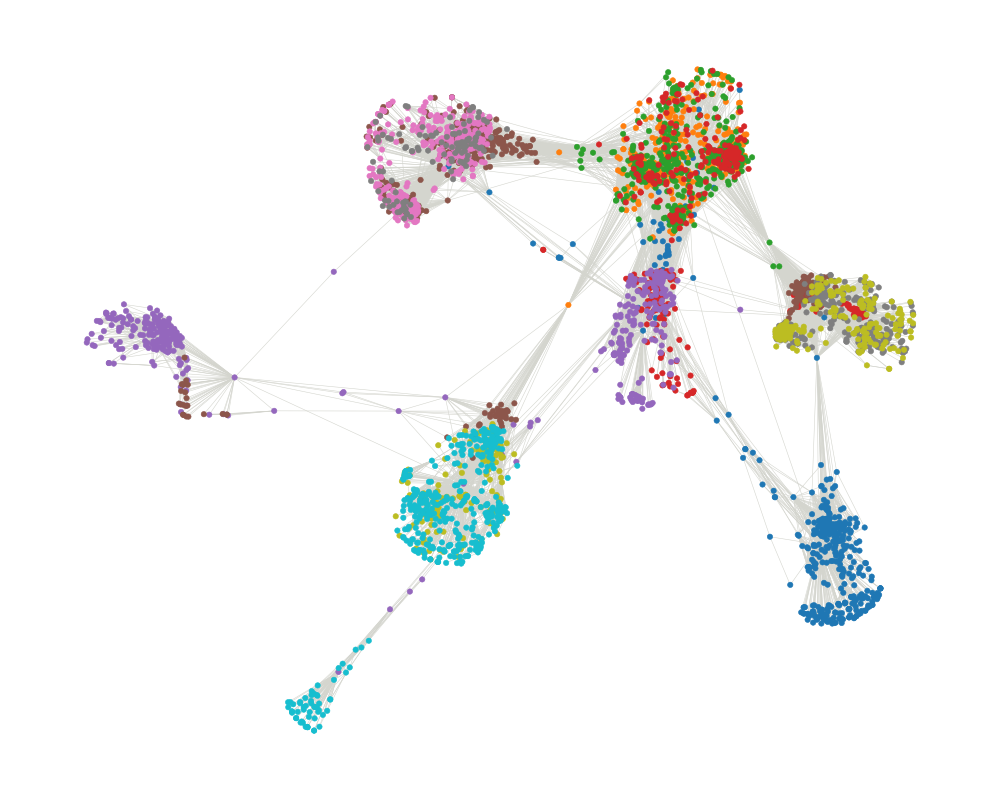
\includegraphics[width=0.7\textwidth]{Graphics/FacebookPoliticalPlot.png}
  \caption{Facebook Graph}
  \label{fig:FacebookGraph}
\end{figure}
\FloatBarrier



Der Graph ähnelt auf den ersten Blick keinem, der bisher generierten Graphen. Zudem fällt aber sofort auf, dass dieser Graph aus deutlich mehr Knoten besteht, zudem weniger Subgraphen besitzt aber dennoch eine grundsätzlich ähnliche Struktur zu unseren anderen Graphen aufweist. Die Berechnungen der Zentralitäten befinden sich ebenfalls auf Github \cite{TZ}, da es sich um zu viele Werte handelt. Nun interessiert uns jedoch, wie diese Zentralitäten verteilt sind und ob dieser Graph die erwarteten Verteilungen nachweist. Nachdem wir den den Graphen \ref{fig:FacebookGraph} durch unsere Methode laufen lassen haben, welche die Plots über die Verteilungen erstellt, sind folgende Diagramme entstanden:

\FloatBarrier
\begin{figure}[h!]%
  \centering
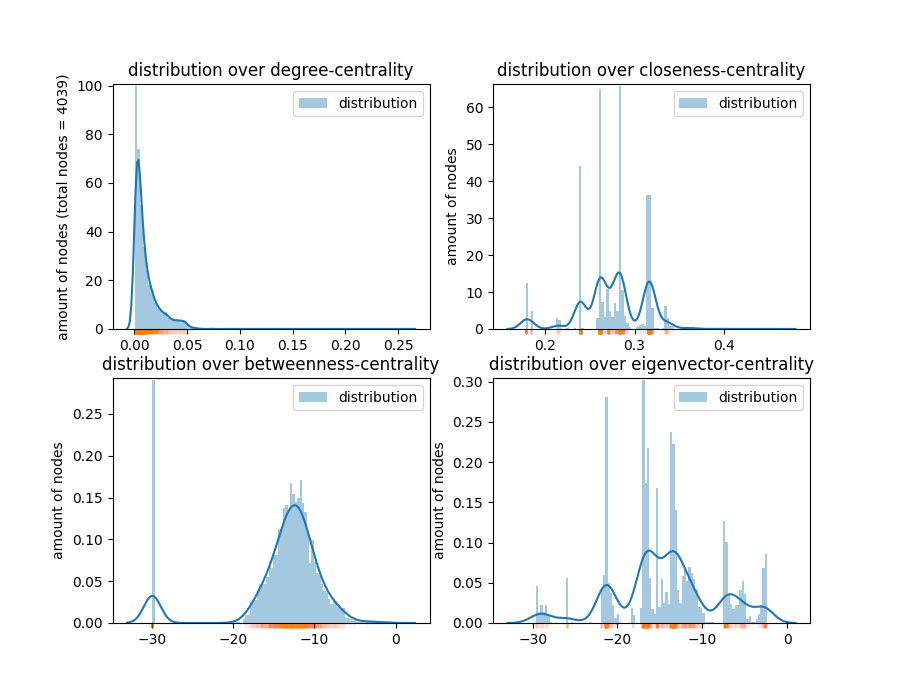
\includegraphics[width=0.8\textwidth]{Graphics/facebookLOG.png}
  \caption{Facebook Graph Distribution}
  \label{fig:FacebookGraphDistribution}
\end{figure}
\FloatBarrier

Sofort fällt auf, dass wir bei keiner Zentralität eine Normalverteilung erkennen. Die \textbf{Grad-Zentralität} fällt uns aber direkt auf, denn es handdelt sich hier um eine Exponentialverteilung. Die anderen Balkendiagramme der \textbf{Betweenness-} und \textbf{Eigenvektor-Zentralität} ähneln jedoch den Verteilungen aus \ref{fig:distributionALL}. Was zudem auffällig ist, dass die Diagramm stark an die Verteilungen von \ref{fig:distributionGOT} erinnern. Auch wenn diese Ergebnisse sehr ernüchtern scheinen und vor allem das Balkendiagramm der \textbf{Nähe-Zentralität} erneut nicht normalverteilt ist, wollen wir uns überlegen, woran dies liegen kann. Bei den anderen Zentarlitäten erkennen wir eine starke Fluktuation der Balken und daher keine schöne Verteilung, die wir aus dem Mathematischen Wahrscheinlichkeitsverteilungen kennen. Visuell fällt jedoch auf, dass der Graph \ref{fig:FacebookGraphDistribution} verglichen mit dem Plot des Graphen \ref{ch:SNA} durchaus Parallelen aufweist. Wir sehen deutliche Ansammlungen von Knoten die auch gut als Teilgraphen bezeichnet werden können. Zwischen den Teilgraphen erkenne wir, so wie bei \ref{fig:SNA}, einige Kanten, die die Teilgraphen untereinander verbinden. Natürlich weist der obige Graph deutlich mehr Kanten und Knoten auf als die bisherigen Graphen. Unsere Graphen haben im Schnitt um die \textbf{950} Knoten und \textbf{8700} Kanten, daher also circa neun mal so viele Kanten wie Knoten. Auch haben wir im Schnitt um die \textbf{10100} Cliquen, welche maximal acht Knoten groß sind. Bei dem Facebook Graphen \ref{fig:FacebookGraph} hingegen sprechen wir von \textbf{4093} Knoten und \textbf{88234} Kanten. Das heißt circa einundzwanzig mal so viele Kanten wie Knoten. Doch wenn wir unsere Kanten und Knoten im Code des Graphen Generators erhöhten, um ebenfalls die selbe Relation zu erhalten, sind alle vier untersuchten Zentralitäten annähern Normalverteilt. Was zum einen daran liegt, dass wir letztendlich Graphen wie \ref{fig:GOT2.0} erhalten, die noch viel dichter besetzt sind und leider alle Knoten mit beinahen allen anderen Knoten verbunden sind, was eher untypisch für \textit{soziale Netzwerke} ist. Wir können aber auf jeden Fall festhalten, dass sich die \textbf{Betweenness-} und \textbf{Eigenvektor-Zentralität} bei allen untersuchten Datensätzen starke Parallelen zu den Verteilungen des generierten sozialen Netzwerk nachweisen. Jedoch wundert uns nach wie vor die Verteilung der \textbf{Gradzentralität}. Daher ist es ratsam, unseren Code und die damit verbundenen Plot so anzupassen, dass es dem Plot \ref{fig:FacebookGraphDistribution} ähnelt. Anschließend können wir die Verteilungen der Zentralitäten betrachten und dadurch eine genauere Aussage erzielen. 


\section{Anpassung des generierten Plots}
Nachdem uns die Verteilungen durchaus gewundert haben, wollen wir den nächsten Plot weitestgehend versuchen an \ref{fig:FacebookGraphDistribution} anzupassen. An dieser Stelle muss durchaus betont werden, dass es sich bei unseren generierten Plot keinesfalls um untypische oder falsche soziale Netzwerke handelt. In diesem Abschnitt wollen wir lediglich eine bessere Vergleichsbasis herstellen. Dies erhalten wir, indem wir zum einen die Anzahl an Cluster auf \textbf{sieben} Stück anpassen und die Anzahl der Knoten pro Cluster erhöhen. Gleichzeitig aber die jeweiligen Größen deutlich mehr variieren lassen und vor allem die Kanten-Menge, also Anzahl an Verbindungen, deutlich erhöhen. Schließlich erhalten wir folgende Graphen: 

\FloatBarrier
\begin{figure}[h!]%
  \centering
  \subfloat[][]{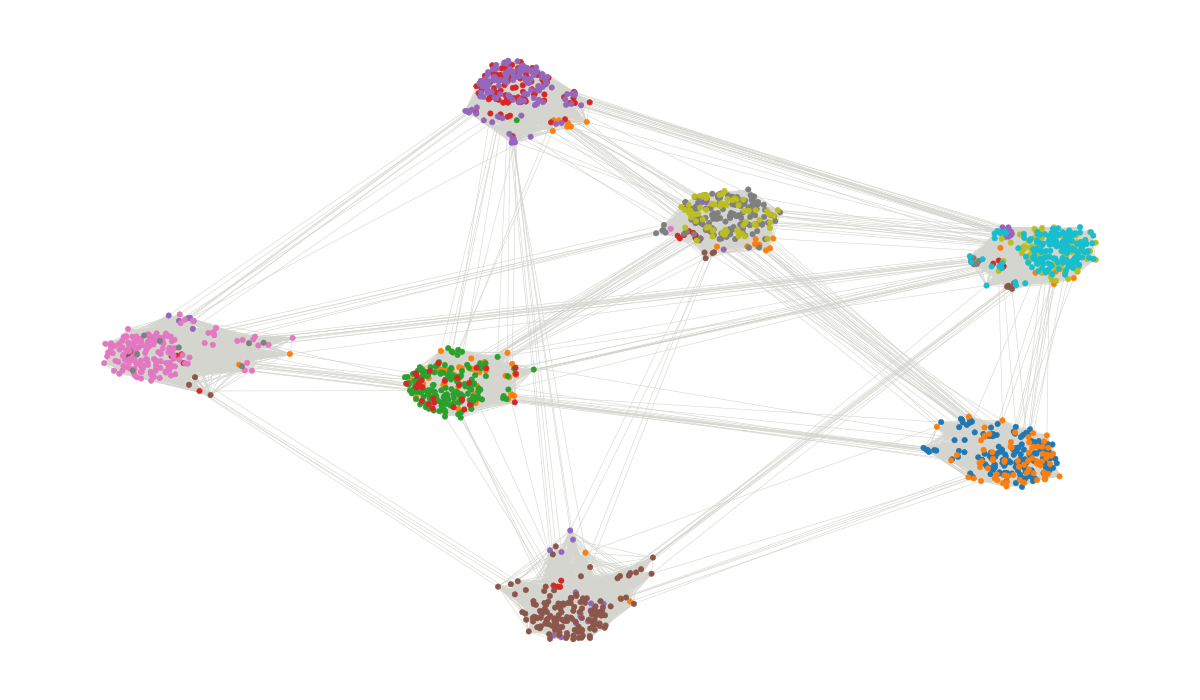
\includegraphics[width=0.8\textwidth]{Graphics/generatedPlotFinal.png}}%
  \qquad
  \subfloat[][]{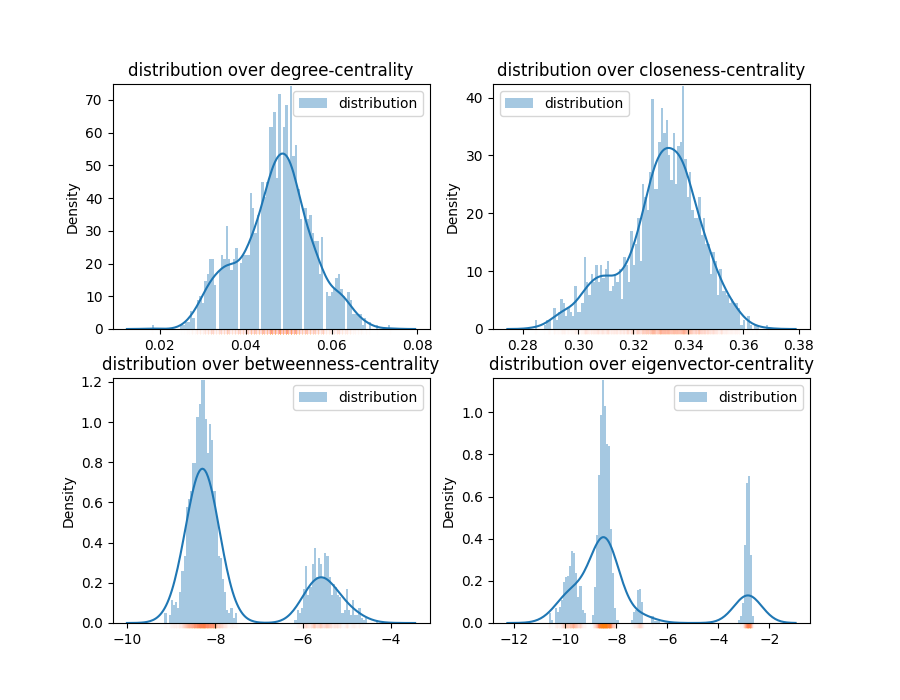
\includegraphics[width=0.7\textwidth]{Graphics/generatedPlotDensity.png}}
  \caption{Final optimierter Graph}
  \label{fig:ourGraphFinalPlot}
\end{figure}
\FloatBarrier

Natürlich sehen wir direkt, ohne die Werte genauer analysiert zu haben, dass wir keinen zu \ref{fig:FacebookGraphDistribution} identischen Graphen erzeugen können. Dies liegt an mehreren Faktoren, die wir auch im Ausblick erörtern möchten. Allgemein sind unsere Graphen, auch wenn wir die Varianz der Graph-Größen best möglichst garantieren wollen, auf den ersten Blick ähnlich groß. Jedoch haben wir bei der Verteilung der Zwischen- und Eigenvektor Zentralität eine absolute Verbesserung erzielen können, indem wir die Zentralitäten, bevor sie geplottet werden, logarithmiert haben. Dies haben wir nachträglich auch bei allen vorherigen Verteilungen gemacht. Dies ermöglicht es uns, die Verteilung auseinander zu zerren, da sich die Werte stets um \textbf{0.0} verteilt haben. Zwar haben wir nun erneut bei \ref{fig:ourGraphFinalPlot} und \ref{fig:FacebookGraphDistribution} keine identischen Verteilungen erzielen können. Tatsächlich können wir dies mathematisch begründen, denn wenn zwei Zufallsvariablen \textbf{X} und \textbf{Y} standardnormalverteilt und unabhängig sind, dann wären für Parameter $\lambda = \frac{1}{2}$ die Variablen $X^2+Y^2$ exponentialverteilt \cite{verteilung}. Doch hat uns die Optimierung in diesem Kapitel dennoch viel gebracht. Unter anderem konnten beweisen, dass wir mit wenigen Anpassungen des Codes, annähernd vergleichbare Verteilungen erhalten. Um den idealen Vergleich herzustellen, müssten wir jedoch größere Änderungen am Code vornehmen, was jedoch nicht mehr im Umfang dieser Arbeit liegt. 

\todo{noch mehr zu Cliquen und Brücken}


